\chapter{Design and Implementation}

\section{Modelling}

\subsection{The Protocol}

\subsection{State Transitions}
Having adapted the protocol, we then had to create a state transition system for
the nodes in your protocol in order to encode it in Disel. For creating the states,
we need to look at what the function of each node is in the protocol at a particular
moment and what type of data it holds at that time.

A node should only be able to transition from one state to another when it either
receives or sends a message. Therefore, the data held by the node in each state
should be enough for it to be able to create the message it wants to send or to
be able to correctly process the message it receives.

We tried to minimise the number of states and transitions between them, in order
to simplify the proof in Disel. This was important because each state transition
has to be shown to hold with the invariant so reducing the state transitions,
reduces the number of proofs.

We decided that a node can either be initialised as an acceptor or a proposer.
The state transitions of each node will depend upon this intial state, so below
we will separately look at the state transition systems for the proposer and the
acceptor.

The main difference between the state transition for the acceptor and the proposer
is that the acceptor sends and receives messages from a single proposer while a
proposer has to send and receive messages from all the acceptors.


\subsubsection{Proposer}
\begin{figure}
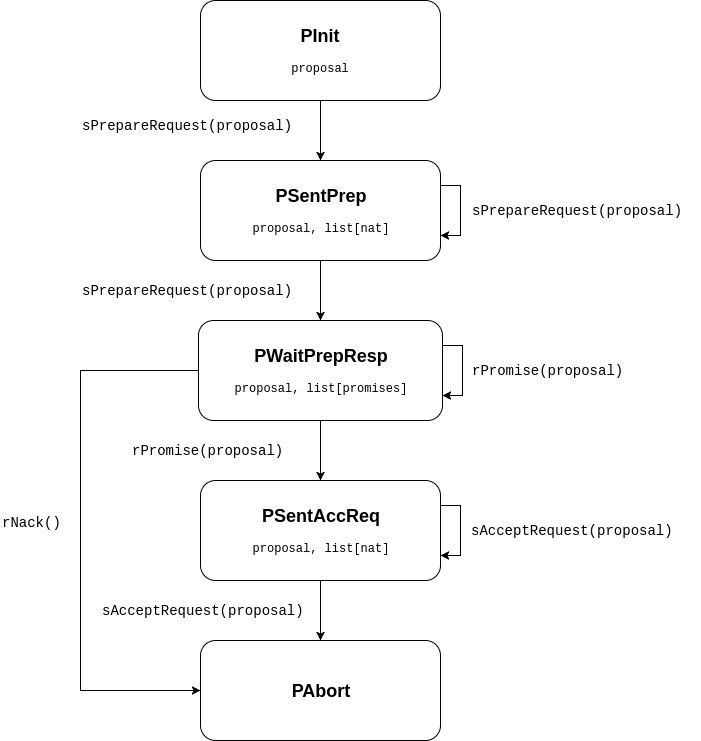
\includegraphics[width=\textwidth]{figures/proposer_state_transitions.png}
\caption{Proposer State Transition Diagram
\label{fig:myInlineFigure}}
\end{figure}

The proposer starts off in the \texttt{PInit} state where it is initialised with
a \texttt{proposal} (a custom defined data type which is tuple of two natural numbers),
$\langle p, v \rangle$.
The natural number $p$ is the proposal number and $v$ is the value that the
proposer tries to achieve consensus on. This means that the first prepare
request this proposer sends will this proposal $\langle p, v \rangle$.

The proposer then moves to the \texttt{PSentPrep} state when it starts to send prepare
requests to the acceptors. In this state, the proposer still holds the proposal
but additionally now also stores a list of natural numbers, \texttt{sent\_to}. This list stores the
natural number identifiers of the acceptors, this proposer has sent requests to.
Whenever it sends a prepare request to an acceptor, it adds the identifier of
the acceptor to this list.
The proposer remains in the \texttt{PSentPrep} state and keeps sending prepare requests
until the contents of \texttt{sent\_to} become equal to the global list \texttt{acceptors} which
holds the identifiers of all the acceptors in the system. This means the proposer
stays in this state until it has sent a prepare request to every single acceptor
in the system.

Once the proposer has sent the last prepare request, it them transitions to
the \texttt{PWaitPrepResp} state. In this state the proposer again holds a proposal and
another list \texttt{promises} which is defined as below to be a list of tuples
each containing a \texttt{nid} (a natural number identifier for a node), a boolean
and a \texttt{proposal}.

\texttt{Definition promises := seq (nid * bool * proposal).}

The proposer stays in this states and keeps receiving messages from the acceptor
until one of the following two things happen:
\begin{enumerate}
  \item It receives a nack response from the acceptor. This indicates that the
    acceptor might already have promised a proposal
    with a proposal number greater than $p$. This leads to the proposer to
    transition into the \texttt{PAbort} state. In this state the proposer basically
    gives up trying to achieve consensus using the proposal number $p$ that it was
    initialised with and completely stops sending and receiving messages. Hence,
    the proposer doesn't need to hold any data in this state.
  \item It receives a promise response from every single acceptor. When this
    happens, the proposer transitions to the \texttt{PSentAccReq} state.
\end{enumerate}

When the proposer reaches the \texttt{PSentAccReq}, it means it has received a promise
from every single acceptor and it can now start sending accept requests to each
of the acceptors in the system. In the \texttt{PSentAccReq} the proposer again stores
a list \texttt{sent\_to} to keep track of every single acceptor it has already sent the
accept request to. It also stores another \texttt{proposal} which is has the same
proposal number $p$ that the proposer was initialised with but the value $v$ is the
the value from the highest numbered proposal it received in a promise response.
In the verification section, we will look at how it determines this value by looping over
the \texttt{promises} list from the \texttt{PWaitPrepResp} state. The sending of
accept requests works similar to sending prepare requests in the
\texttt{PSentPrep} state. Finally, when the proposer finishes sending the
accept requests to all the acceptors, it transitions to the \texttt{PAbort}
state where it stops sending and receiving messages.


\subsubsection{Acceptor}
\begin{figure}
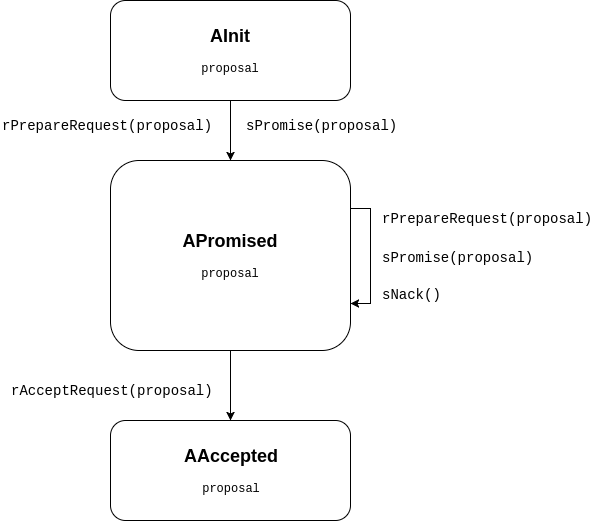
\includegraphics[width=\textwidth]{figures/acceptor_state_transitions.png}
\caption{Acceptor State Transition Diagram
\label{fig:myInlineFigure}}
\end{figure}

The Acceptor starts off in the \texttt{AInit} state. It doesn't hold any data
in this state as it is not sending any messages. It keeps listening for messages
and on receiving a prepare request message, it transitions to \texttt{APromised}
state.

In the \texttt{APromised} state, the acceptor holds a \texttt{proposal}. This is
the highest numbered proposal that it has received so far in a prepare request
message. In this state, on receiving a prepare request, if the proposal number
of the proposal in the prepare request is greater than the proposal number of
the proposal it currently holds, it updates its current state to hold the new
proposal but still remains in the \texttt{APromised} state. If the proposal
number of the proposal in the prepare request is not greater, the acceptor
sends a nack response to the proposer who sent the prepare request and does not
update its state.

In the \texttt{APromised}, on receiving an accept request, if and only if
the value of the proposal number proposal in the accept request is greater than
the proposal number of the proposal that it currently holds, it transitions to the
\texttt{AAccepted} state where it now holds the new proposal with the greater
proposal number. If the proposal number of the new proposal number is not greater,
the acceptor remains in the same state.

In the \texttt{AAccepted} state, the acceptor stops listening for and responding
to messages. This is similar to the \texttt{PAbort} state for the proposer.


\subsection{Inductive Invariant}

\section{Verification}
